\chapter{局所量子場と一次元ディラック方程式}

我々はすでに、量子場をその量子、生成消滅演算子、そして非相対論的粒子に対する最も単純なハミルトニアンを通して見てきた。ここではその仕組みを実際に働かせてみよう。まず、空間的に局所的なハミルトニアンがどのように運動量を保存するかを、単に主張するのではなく、実際に見る。次に、場の積が散乱と崩壊を記述することを見て、ハミルトニアンの繰り返し作用が図式的摂動論の初歩を生み出すのを眺める。その後になって初めて、約束したフェルミオンの問題に取り掛かる。最も明快な入口は、まだフェルミオン場ではなく、一次元ディラック方程式である。

\section{場のハミルトニアンをもう一度}

一種類の非相対論的粒子に対するハミルトニアンを次のように書く。
\begin{equation}
H_0=\int dx\,
\psi^\dagger(x)
\left[-\frac{\partial_x^2}{2m}+V(x)\right]
\psi(x).
\label{eq:l9-nonrel-hamiltonian}
\end{equation}
この記法は一次元に見えるが、冒頭の議論はその制限に依存しない。三次元では、\(x\)はベクトル\(\mathbf{x}\)を表し、\(dx\)は\(d^3x\)を、\(-\partial_x^2\)は\(-\nabla^2\)を表すことができる。

演算子\(\psi^\dagger(x)\)は\(x\)に粒子を生成し、\(\psi(x)\)はそこにある粒子を消滅させる。それらの正規順序積
\begin{equation}
n(x)=\psi^\dagger(x)\psi(x)
\end{equation}
は局所数密度である。したがってポテンシャル項は
\begin{equation}
H_V=\int dx\,V(x)n(x).
\end{equation}
と書ける。これはまさに古典気体に対して書くものと同じである。\(x\)の近くの粒子を数え、それぞれにポテンシャルエネルギー\(V(x)\)を割り当て、空間について足し合わせる。この段階では粒子は互いに相互作用しない。外部から課されたポテンシャルに応答することはあるが、それ以外にハミルトニアンは独立な一粒子エネルギーの和である。

単純化してから逆戻りするのが有用である。ポテンシャルを定数\(V(x)=V_0\)とする。定数ポテンシャルは力を及ぼさないが、その演算子としての意味は明白である。
\begin{equation}
\begin{aligned}
H_V&=V_0\int dx\,\psi^\dagger(x)\psi(x)=V_0N,\\
N&=\int dx\,n(x).
\end{aligned}
\end{equation}
これは各粒子に同じ付加エネルギーを与える。非相対論的記述で静止エネルギーを保つには、\(V_0=mc^2\)と選ぶ。するとこの項は粒子一つあたり静止エネルギー一つを数える。この他には退屈な定数を保持するのは、それが並進不変性を保ち、数え上げ操作を可視化するからである。

\section{更新規則としてのハミルトニアン}

運動量が保存されるとはどういうことか。その答えは、ハミルトニアンが何をするかという観点から述べるべきである。\(\psi\) を場の演算子、一粒子波動関数、多体状態のすべてに同時に使うことを避けるため、多体状態を \(\lvert\Phi(t)\rangle\) と呼ぶことにしよう。短い区間 \(\epsilon\) の間に、
\begin{equation}
\lvert\Phi(t+\epsilon)\rangle
=\left(1-i\epsilon H+O(\epsilon^2)\right)
\lvert\Phi(t)\rangle,
\label{eq:l9-short-update}
\end{equation}
ここで \(\hbar=1\) である。変化しない状態が第一項であり、最初の補正は \(H\) によって生成される。この更新を繰り返すことが Schr\"odinger 方程式である。

運動量保存は今や具体的な意味を持つ。初期状態が確定した全運動量\(P\)を持つならば、\(H\lvert\Phi\rangle\)も同じ全運動量を持たねばならない。他の性質は変化しうるし、個々の粒子は運動量を交換しうるが、ハミルトニアンが状態を異なる全\(P\)を持つセクターへ移すことはできない。これはハミルトニアンを運動量基底で書き直すことによって直接確かめられる。

\section{運動量のデルタ関数としての空間積分}

フーリエの規約を
\begin{align}
\psi(x)&=\int\frac{dp}{\sqrt{2\pi}}\,a(p)e^{ipx},\\
\psi^\dagger(x)&=\int\frac{dq}{\sqrt{2\pi}}\,a^\dagger(q)e^{-iqx}.
\label{eq:l9-field-fourier}
\end{align}
と選ぶ。演算子\(a(p)\)は運動量\(p\)の粒子を消滅させる。演算子\(a^\dagger(q)\)は運動量\(q\)の粒子を生成する。異なる文字を使うことが本質的である。二つの運動量は、空間積分がそれらを関係づけるまで独立に積分される。

数演算子の項から始める。
\begin{align}
N
&=\int dx\,\psi^\dagger(x)\psi(x)\\
&=\int\frac{dp\,dq}{2\pi}\,
a^\dagger(q)a(p)
\int dx\,e^{i(p-q)x}.
\end{align}
残りの積分は
\begin{equation}
\int dx\,e^{i(p-q)x}=2\pi\delta(p-q).
\end{equation}
である。\(p\ne q\)に対しては、位相が振動し、正と負の寄与の間で相殺される。\(p=q\)に対しては、まったく振動しない。ディラックのデルタ分布は、これら二つの事実を組み合わせる正確な対象である。したがって、
\begin{align}
N
&=\int dp\,dq\,a^\dagger(q)a(p)\delta(p-q)\\
&=\int dp\,a^\dagger(p)a(p).
\label{eq:l9-number-momentum}
\end{align}
この演算子は運動量\(p\)の粒子を取り除き、まったく同じ運動量の粒子を一つ戻す。決定的な要素は\(x\)に関する積分であった。それが、入る運動量と出る運動量の等しさを強制するデルタ関数を生み出した。

\begin{classroomqa}
\lecturetimestamp{00:17:02}
\audiencequestion{\(p=q\)のときに現れる無限大はどうなったのか。}
\lecturerresponse{デルタ関数はその高さを評価することによって使われるのではない。それは積分によって定義される分布である。\(\int dk\,\delta(k)f(k)=f(0)\)。「``無限に高く、無限に狭い''」という表現は、その積分された重みが1であることを思い出させるだけである。ここでは、\(p-q=0\)とせよと指示しており、無限の答えは残らない。}
\end{classroomqa}

同じ機構は、はるかに一般的な局所単項式に対しても働く。ある項がいくつかの消滅場といくつかの生成場を含み、それらが異なる種に属していてもよいが、すべて一点で評価され、その点について積分されるとしよう：
\begin{equation}
\int dx\,
\prod_{r=1}^{n} \psi_{i_r}^\dagger(x)
\prod_{s=1}^{m} \psi_{j_s}(x).
\end{equation}
消滅する粒子が運動量\(p_s\)を運び、生成される粒子が運動量\(q_r\)を運ぶとする。フーリエ展開により
\begin{equation}
\int dx\,
e^{i(\sum_s p_s-\sum_r q_r)x}
=2\pi\,
\delta\!\left(\sum_s p_s-\sum_r q_r\right).
\label{eq:l9-total-momentum-delta}
\end{equation}
が得られる。この結果は\(p_1\)を\(q_1\)と、\(p_2\)を\(q_2\)と、以下同様に、対にするのではない。それはただ
\begin{equation}
\sum_{\mathrm{annihilated}}p
=
\sum_{\mathrm{created}}q.
\end{equation}
を課すだけである。これはまさに相互作用に要求される規則である：個々の運動量は変化してよいが、全運動量は変化しない。より深い言明は並進不変性である。各点で同じ重みで積分された局所密度には特別な原点がなく、そのフーリエ変換は対応する運動量保存のデルタ関数を運ぶ。

\begin{classroomqa}
\lecturetimestamp{00:23:04}
\audiencequestion{提案されたハミルトニアン項は本当にこれらすべての場の演算子の積なのか。なぜそのような積を書くのか。}
\lecturerresponse{はい。この積は、どの粒子が一点で取り除かれ、どの粒子が生成されるかを指定する。その物理的動機は観測された散乱または崩壊過程から来るであろう。運動量の議論を先に確立しておくことで、それらの相互作用を直ちに読み取ることができる。}
\end{classroomqa}

\section{運動量空間と位置空間における運動エネルギー}

次に同じ仕組みを微分項に適用する。微分は平面波に作用する：
\begin{equation}
-\partial_x^2 e^{ipx}=p^2e^{ipx}.
\end{equation}
したがって
\begin{align}
H_{\mathrm{kin}}
&=\int dx\,\psi^\dagger(x)
\left(-\frac{\partial_x^2}{2m}\right)\psi(x)\\
&=\int dp\,\frac{p^2}{2m}\,a^\dagger(p)a(p).
\label{eq:l9-kinetic-momentum}
\end{align}
ここでも空間積分が入射運動量と出射運動量の等しさを強制する。新しい因子\(p^2/2m\)は、各運動量モードの粒子数をそのモードの運動エネルギーで重み付けするだけである。

\begin{classroomqa}
\lecturetimestamp{00:24:46}
\audiencequestion{平面波を二回微分すると負符号が付くべきか。}
\lecturerresponse{はい、\(\partial_x^2e^{ipx}=-p^2e^{ipx}\)。ハミルトニアンにはすでに補償する負符号が含まれているので、\(-\partial_x^2\)は正の固有値\(p^2\)を持つ。}
\end{classroomqa}

\begin{classroomqa}
\lecturetimestamp{00:27:20}
\audiencequestion{運動エネルギーが保存されるのはポテンシャルが定数のときだけか。}
\lecturerresponse{はい。位置に依存するポテンシャルがなければ力はなく、運動エネルギーは別個に保存される。非定数の外部ポテンシャルでは、全ハミルトニアンが陽に時間依存しなければ、運動エネルギーとポテンシャルエネルギーは交換し合いながら全ハミルトニアンは保存される。}
\end{classroomqa}

\begin{classroomqa}
\lecturetimestamp{00:27:42}
\audiencequestion{運動量空間の運動ハミルトニアンにおいて\(\psi^\dagger\psi\)の役割は何か。}
\lecturerresponse{それは数え上げ演算子である。モード積\(a^\dagger(p)a(p)\)は運動量\(p\)の粒子を数え、因子\(p^2/2m\)はそれぞれに適切な運動エネルギーを割り当てる。}
\end{classroomqa}

正値性を見る第二の方法がある。一度部分積分し、境界項を無視すると
\begin{align}
\int dx\,\psi^\dagger(-\partial_x^2)\psi
&=\int dx\,(\partial_x\psi^\dagger)(\partial_x\psi).
\label{eq:l9-positive-kinetic}
\end{align}
が得られる。無限遠で適切に消える場、または周期的境界条件では、境界からの寄与はゼロである。結果は絶対値の二乗の形をしており、非負である。それはまた場の理論に共通するパターンを示している：エネルギーは場の空間微分の二乗を含む。

\section{局所接触相互作用}

ここで場の積に物理的な仕事を与えよう。二つの種を考え、描像を親しみやすく保つためだけにそれらを電子と陽子と呼ぶ。当面それらは意図的に偽物である：どちらもボソン演算子で扱われ、それらの真のクーロン相互作用は省略される。それらの自由ハミルトニアンは
\begin{equation}
H_0=\int dx\left[
\psi_e^\dagger\left(-\frac{\partial_x^2}{2m_e}\right)\psi_e
+
\psi_p^\dagger\left(-\frac{\partial_x^2}{2m_p}\right)\psi_p
\right].
\end{equation}
モデル相互作用
\begin{equation}
H_{\mathrm{contact}}
=g\int dx\,
\psi_e^\dagger(x)\psi_p^\dagger(x)
\psi_e(x)\psi_p(x).
\label{eq:l9-contact}
\end{equation}
を加える。これを右から左へ読む。それは同じ点\(x\)にある電子と陽子を探し、それらを消滅させ、その点で両方を再生成する。二つの粒子が一緒になければ、この局所項はゼロを与える。それらの世界線が出会えば、全運動量を保存しながら個々の運動量を変えうる。したがってそれは理想化されたゼロ距離散乱ポテンシャルとして働く。

\begin{figure}[htbp]
\centering
\includegraphics[width=0.94\linewidth]{lecture_09_frame_02.png}
\caption{黒板上の接触相互作用。四つの局所場演算子が時空のスケッチの上に現れ、出会いの点が理想化された相互作用が作用する唯一の場所である。}
\lectureframe{00:35:36}
\end{figure}

\begin{figure}[htbp]
\centering
\begin{tikzpicture}[x=1.2cm,y=1.0cm,>=Latex]
\draw[->] (-3.0,0) -- (3.0,0) node[right] {$x$};
\draw[->] (0,-0.2) -- (0,4.2) node[above] {$t$};
\coordinate (v) at (0,2.0);
\fill (v) circle (1.8pt);
\draw[thick,->] (-2.2,0.4) -- (v);
\draw[thick,->] (2.0,0.4) -- (v);
\draw[thick,->] (v) -- (-1.6,3.7);
\draw[thick,->] (v) -- (2.2,3.7);
\node[left] at (-1.65,0.7) {$e$};
\node[right] at (1.55,0.7) {$p$};
\node[left] at (-1.15,3.3) {$e$};
\node[right] at (1.65,3.3) {$p$};
\node[right] at (0.12,2.05) {$g$};
\end{tikzpicture}
\caption{局所散乱描像の明快な再構成。頂点は式~\eqref{eq:l9-contact}の演算子の略記であり、古典的な衝突法則ではない。}
\end{figure}

実際の電子と陽子はクーロンポテンシャルを通じて遠隔的に相互作用する。接触モデルは最初の短い一歩にすぎない：もし実験が二つの種が重なるときにのみ散乱することを示すなら、式~\eqref{eq:l9-contact}はハミルトニアンに置くであろう種類の項である。

\begin{classroomqa}
\lecturetimestamp{00:35:40}
\audiencequestion{エネルギーが変化しないのなら、なぜこの散乱演算子はハミルトニアンの一部なのですか。}
\lecturerresponse{ハミルトニアンはエネルギー演算子であると同時に、状態を変化させる生成子でもある。二つの粒子間のポテンシャルエネルギーは、時間発展の下で散乱を引き起こす。全エネルギーの保存は、状態や粒子の個々の運動量が変わらないことを意味しない。}
\end{classroomqa}

これで実用的な規則が得られる。まず、粒子がどのような局所過程を経ることができるかを実験から学ぶ。次に、それらの過程を状態を更新する演算子に符号化する。場の積は装飾的な代数ではない。そのダガー付き因子とダガーなし因子が、どの種が現れ、どの種が消えるかを指定する。

\section{崩壊、逆過程、エルミート性}

泡箱が種\(A\)の飛跡を明らかにし、それが終わる点から飛跡\(B\)と\(C\)が現れるとしよう。局所過程は
\begin{equation}
A\longrightarrow B+C.
\end{equation}
であり、それを実行する演算子は
\begin{equation}
V=g\int dx\,
\psi_B^\dagger(x)\psi_C^\dagger(x)\psi_A(x).
\label{eq:l9-decay-half}
\end{equation}
である。消滅場が\(A\)を除去し、二つの生成場が同じ点で\(B\)と\(C\)を生成する。すべての\(x\)にわたって等しい重みで積分することは空間並進不変性を表し、直ちに
\begin{equation}
p_A=p_B+p_C.
\end{equation}
を与える。

ハミルトニアンはエルミートでなければならない。これが\(e^{-itH}\)をユニタリにし、全確率を保存する。式~\eqref{eq:l9-decay-half}はそれ自体ではエルミートではないので、その随伴を加えなければならない。
\begin{equation}
H_{\mathrm{int}}
=\int dx\left[
g\,\psi_B^\dagger\psi_C^\dagger\psi_A
+g^*\,\psi_A^\dagger\psi_C\psi_B
\right](x).
\label{eq:l9-hermitian-vertex}
\end{equation}
実結合定数\(g\)に対して、二つの係数は同じである。エルミート共役は、ダガー付き場とダガーなし場を交換するだけでなく、演算子の順序も逆にする。このボソン的玩具模型では、異なる種の場は可換であるため、その反転は追加の複雑さを引き起こさない。

第二項は逆過程
\begin{equation}
B+C\longrightarrow A.
\end{equation}
を実行する。したがって、崩壊を許す閉じたユニタリなハミルトニアンは、再結合振幅も含む。これは、選ばれた外部運動量のあらゆる組に対して両方向が起こることを約束するものではない。エネルギーやその他の保存則が、一方の方向を運動学的に到達不可能にするかもしれない。これは、演算子とその随伴の両方が力学に属することを述べている。

\begin{classroomqa}
\lecturetimestamp{00:42:48}
\audiencequestion{逆過程も許されるという規則に例外はあり得ますか。}
\lecturerresponse{エルミートな閉じた系のハミルトニアンのレベルでは、例外はない。随伴相互作用が必要である。特定の逆反応は依然として運動学や別の保存量子数によって遮断され得るが、共役行列要素は存在する。}
\end{classroomqa}

数\(g\)は結合定数である。\(g\)が小さければ、出会った粒子は弱くしか相互作用しない。大きければ、遷移振幅はより大きい。結合定数は通常、実験で測定されるパラメータであるが、対称性が一見異なるいくつかの結合定数を関係づけることもある。

同じ文法がより複雑な反応も扱う。ベータ崩壊では、
\begin{equation}
n\longrightarrow p+e^-+\bar\nu_e,
\end{equation}
模式的な局所項は四つの場を含む。一つは中性子を消滅させ、三つは陽子、電子、電子反ニュートリノを生成し、さらにエルミート共役な過程も含む。これで、少数の演算子単項式がどのように量子場の理論を定義し始めるかを見るのに十分である。

\section{なぜハミルトニアンの二乗が重要か}

短時間の公式\eqref{eq:l9-short-update}は\(\epsilon\)の一次までしか保っていなかった。完全な展開は
\begin{equation}
e^{-i\epsilon H}
=1-i\epsilon H-\frac{\epsilon^2}{2}H^2
+\frac{i\epsilon^3}{3!}H^3+\cdots.
\label{eq:l9-exponential}
\end{equation}
である。二次ではハミルトニアンが二度作用する。これが最初の複合過程の図の代数的起源である。

頂点\(A\leftrightarrow B+C\)に対して、一回の作用で\(B+C\)を\(A\)に結合でき、二回目の作用でその\(A\)を再び\(B+C\)に分けることができる。
\begin{equation}
B+C\longrightarrow A\longrightarrow B+C.
\label{eq:l9-bc-scattering}
\end{equation}
正味の寄与は\(B+C\to B+C\)散乱振幅である。中間\(A\)は追加の観測事象ではなく、相互作用の二回の作用の間に和をとられる状態を表す。

\begin{classroomqa}
\lecturetimestamp{00:49:54}
\audiencequestion{書き下された二次の積において\(C\)場はダガーを持つべきですか。}
\lecturerresponse{はい、演算子の順序は述べられた順序と一致しなければならない。第一の頂点は\(B\)と\(C\)を消滅させ、\(A\)を生成する。第二の頂点は\(A\)を消滅させ、\(B\)と\(C\)を再生成する。対応するダガーを正しく書くことで、その解釈が回復される。}
\end{classroomqa}

\begin{figure}[htbp]
\centering
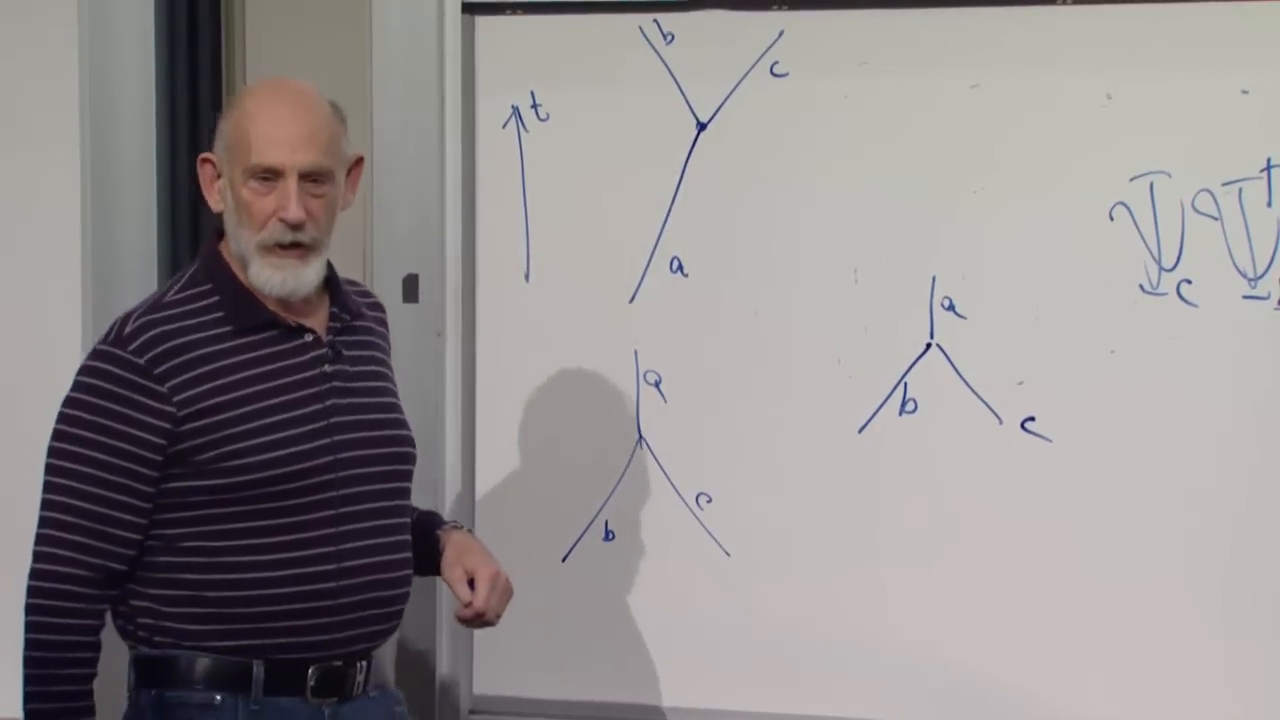
\includegraphics[width=0.94\linewidth]{lecture_09_frame_05.png}
\caption{黒板上の基本\(A\leftrightarrow B+C\)頂点の二つの向き。それらを並置することが、式~\eqref{eq:l9-bc-scattering}の二次過程の視覚的略記である。}
\lectureframe{00:48:56}
\end{figure}

ここで spectator \(B\) を追加する。1つの作用により \(A\) が \(C\) を放出して \(B\) になり、後の作用によりその \(C\) が元の \(B\) と結合して \(A\) を形成する。外部粒子は再び \(A+B\) であるが、それらの運動量は変化しうる。これを \(A\) と \(B\) の \(C\) の交換による散乱と呼ぶ。

\begin{figure}[htbp]
\centering
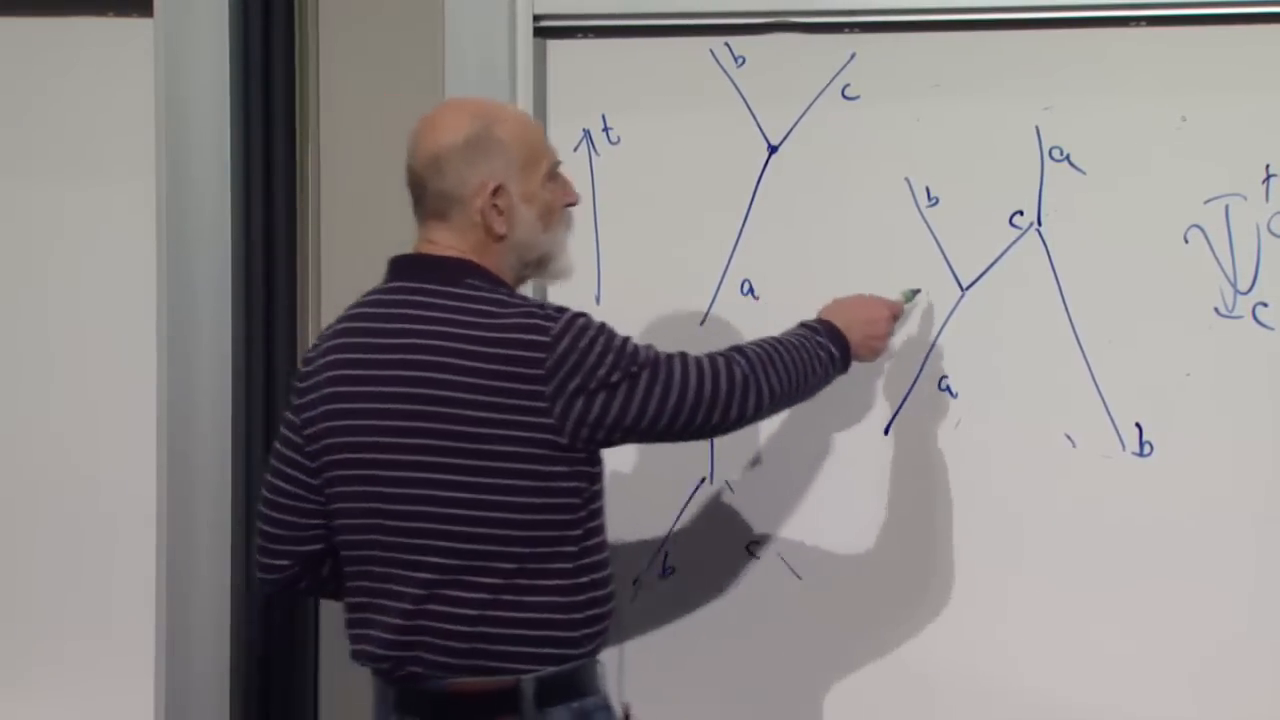
\includegraphics[width=0.94\linewidth]{lecture_09_frame_06.png}
\caption{黒板上の交換構成。右側の図は2つの素過程の頂点を内部 \(C\) 線で結び、外部の \(A\) 粒子と \(B\) 粒子が散乱する。}
\lectureframe{00:51:22}
\end{figure}

\begin{figure}[htbp]
\centering
\begin{tikzpicture}[x=1.1cm,y=1cm,>=Latex]
\draw[->] (-3.7,-0.2) -- (-3.7,4.2) node[above] {$t$};
\coordinate (v1) at (-0.9,1.25);
\coordinate (v2) at (0.9,2.95);
\fill (v1) circle (1.7pt);
\fill (v2) circle (1.7pt);
\draw[thick,->] (-2.6,0.2) -- (v1) node[midway,below left] {$A$};
\draw[thick,->] (2.6,0.2) -- (v2) node[midway,below right] {$B$};
\draw[thick,->] (v1) -- (-2.4,4.0) node[midway,left] {$B$};
\draw[thick,->] (v2) -- (2.5,4.0) node[midway,right] {$A$};
\draw[thick,->,dashed] (v1) -- (v2) node[midway,above left] {$C$};
\node[below] at (0,-0.05) {$A+B\rightarrow A+B$};
\end{tikzpicture}
\caption{\(C\) 交換の明快な再構成。各点は \(g\) の因子を一つ寄与するので、この二次の項は \(g^2\) に比例する。}
\end{figure}

各局所相互作用点を頂点と呼ぶ。各頂点はその結合定数の因子を寄与するので、二頂点の寄与は \(g^2\) を、三頂点の寄与は \(g^3\) を、以下同様に伴う。したがってハミルトニアンの一つの項は反応の大きな族を関連づける。この経済性は量子場の理論がこれほど強力である一つの理由である。少数の局所相互作用が膨大な散乱データを組織する。

\begin{classroomqa}
\lecturetimestamp{00:53:14}
\audiencequestion{過程 \(A\to B+C\to A\) を何と呼ぶか。}
\lecturerresponse{それは自己エネルギー寄与である。測定される \(A\) は裸の1粒子基底状態にすぎないのではない。相互作用する状態は近傍の \(B+C\) 成分の振幅も持つ。それからの散乱はその dressed 構造を明らかにしうる。}
\end{classroomqa}

量子電磁力学がよく知られた例を与える。局所的な電子--光子頂点は電子を消滅させ、電子を再生成し、光子を生成することができる。二次では、電子は光子を放出して再吸収してもよい。これを小さな映画のように語りたくなるが、その規律ある意味は摂動展開における一つの項である。物理的電子は光子を含む成分をもつ dressed 状態である。

この成分が ``約1パーセント'' であるという教室での見積もりは、微細構造定数 \(\alpha_{\mathrm{em}}\simeq 1/137\) が定める尺度を伝える。光子 Fock 成分の正確な確率はエネルギー分解能と相互作用状態の定義に依存し、孤立電子の普遍的な1パーセントの性質ではない。堅牢な主張は、相互作用が電子の測定可能な構造を変えるということである。

\section{図が語ることと語らないこと}

図は相互作用ハミルトニアンの冪のための計算上の略記である。それらは粒子が確実に1つの事象を行い、次に別の事象を行うという信頼できる古典的履歴ではない。どの中間的選択肢 ``が実際に起こったか'' を決めようと内部を覗くことは、通常の量子干渉と同様に、実験を変え、コヒーレントな和を破壊する。

\begin{classroomqa}
\lecturetimestamp{00:56:52}
\audiencequestion{最初の頂点でエネルギーと運動量の両方が保存されるか。}
\lecturerresponse{ここで行った等時刻ハミルトニアン構成では、空間積分は直ちに運動量デルタ関数を生じる。その孤立した挿入に対して時間積分はまだエネルギーデルタ関数を生じていない。完全な時間並進不変散乱振幅は全エネルギーを保存するが、中間線は観測粒子のオンシェル関係に従う必要はない。共変的図の言語では各頂点で4元運動量が保存されるが、内部粒子はオフシェルでありうる。}
\end{classroomqa}

素朴な頂点描像における見かけのエネルギー欠損は、相互作用エネルギーを捨ててはならないというもう一つの警告である。全ハミルトニアンは自由粒子エネルギーの和以上のものである。混乱が生じたなら、式~\eqref{eq:l9-exponential}に戻れ。この描像はユニタリ時間発展の展開における一つの項を表している。完全なファインマン図の技術は系統的な時間順序、伝播関数、積分、対称因子を与えるが、基本的な物理はここから始まる。

ある拡張された質問は、放出された光子をゆっくり動く電子の周囲の電場と比較することにより、図をあまりに文字通りに押しすぎている。

\begin{classroomqa}
\lecturetimestamp{00:58:26}
\audiencequestion{電子の距離における電場は、文字通り放射された光子によって生成されるのか。それは干渉やアハラノフ--ボーム効果とどう整合するのか。}
\lecturerresponse{静的場または誘導場は、実光子の流れではない。量子電磁力学は放射と電子の電磁的 dressing の両方を同じ場で記述するが、対応する量子状態と運動学は異なる。超相対論的電子では、一部の場の成分はほぼ実光子の流れのように有用に振る舞うことができる。遅い電子では、文字通りの光子の軌跡は誤ったモデルである。二重スリット干渉とアハラノフ--ボーム効果もまた非古典的な場の現象であるが、それらはこの自己エネルギー図を機械的な映画に変えるものではない。}
\end{classroomqa}

\begin{classroomqa}
\lecturetimestamp{01:01:28}
\audiencequestion{なぜ図の古典的モデルは正確には失敗するのか。}
\lecturerresponse{計算は許されたすべての中間選択肢からの振幅をコヒーレントに加えるからである。経験は図を直観的にするが、その文字通りの内容はそれを定義する演算子展開を決して超えない。それらは \(H^2,H^3,\ldots\) を計算するための簡潔な方法であり、観測された中間事象の記録ではない。}
\end{classroomqa}

\begin{classroomqa}
\lecturetimestamp{01:03:04}
\audiencequestion{通常のクーロン相互作用は光子交換の古典的極限として現れうるか。}
\lecturerresponse{はい。適切な光子媒介振幅を評価し、非相対論的静的極限を取るとクーロンポテンシャルが得られる。その導出は現在の演算子の概略よりも技術的であり、それでもなお光子が文字通り2つの古典的粒子の間を跳ぶものとして読まれるべきではない。}
\end{classroomqa}

\begin{classroomqa}
\lecturetimestamp{01:03:44}
\audiencequestion{結合定数は場の積から計算されるのか。}
\lecturerresponse{通常、それらの数値は実験的入力である。対称性はそれらを制約したり、そうでなければ独立であろう結合を関係づけたりすることができる。そのような関係が異なる反応の相対的強度を予測し、実験がそれを確認するとき、一致は特に有益である。}
\end{classroomqa}

\begin{classroomqa}
\lecturetimestamp{01:04:48}
\audiencequestion{偶発的対称性はゲージ対称性と比べてどのような役割を果たすのか。}
\lecturerresponse{ゲージ対称性は許される構造と結合間の関係を直接制約する。偶発的対称性は基礎的レベルで課されるものではないが、すべての低次で許される相互作用がたまたまそれを尊重するために現れる。それは依然として重要な帰結を持ちうるが、その起源と頑健性はゲージ対称性のそれとは異なる。}
\end{classroomqa}

非相対論的場の理論は今のところこれで十分である。我々はフェルミオンを約束した。それらを直ちに第二量子化するのではなく、まずそれらの場の演算子が満たさなければならない相対論的一粒子方程式を理解しよう。

\section{なぜ電子は相対論を必要とするのか}

まず一次元空間から始める。これは現実的な制限ではないが、三次元スピンの幾何学的複雑さを取り除きつつ、本質的な代数を保つことができる。電子は軽いので、原子の中でも相対論が重要になる。水素中でのその特徴的な速度は
\begin{equation}
v\sim\alpha_{\mathrm{em}}c\approx 0.007c,
\end{equation}
の程度であり、光速のおよそ1パーセントである。重い原子の内殻電子では、その粗い目安は \(v\sim Z\alpha_{\mathrm{em}}c\) となるので、相対論的補正はかなり大きくなりうる。歴史的な興味が決定的な動機であったか、原子の精度がそうであったかに関わらず、相対論的な Schr\"odinger 型方程式は物理的に必要である。

通常の量子化レシピはエネルギーと運動量の古典的関係から始まる。非相対論的には、
\begin{equation}
E=\frac{p^2}{2m},
\end{equation}
であり、置換
\begin{equation}
E\mapsto i\partial_t,
\qquad
p\mapsto-i\partial_x
\end{equation}
により
\begin{equation}
i\partial_t\varphi(x,t)
=-\frac{1}{2m}\partial_x^2\varphi(x,t).
\end{equation}
が得られる。

相対論では代わりに、\(c=1\) として、
\begin{equation}
E^2=p^2+m^2.
\label{eq:l9-rel-dispersion}
\end{equation}
が与えられる。

\begin{figure}[htbp]
\centering
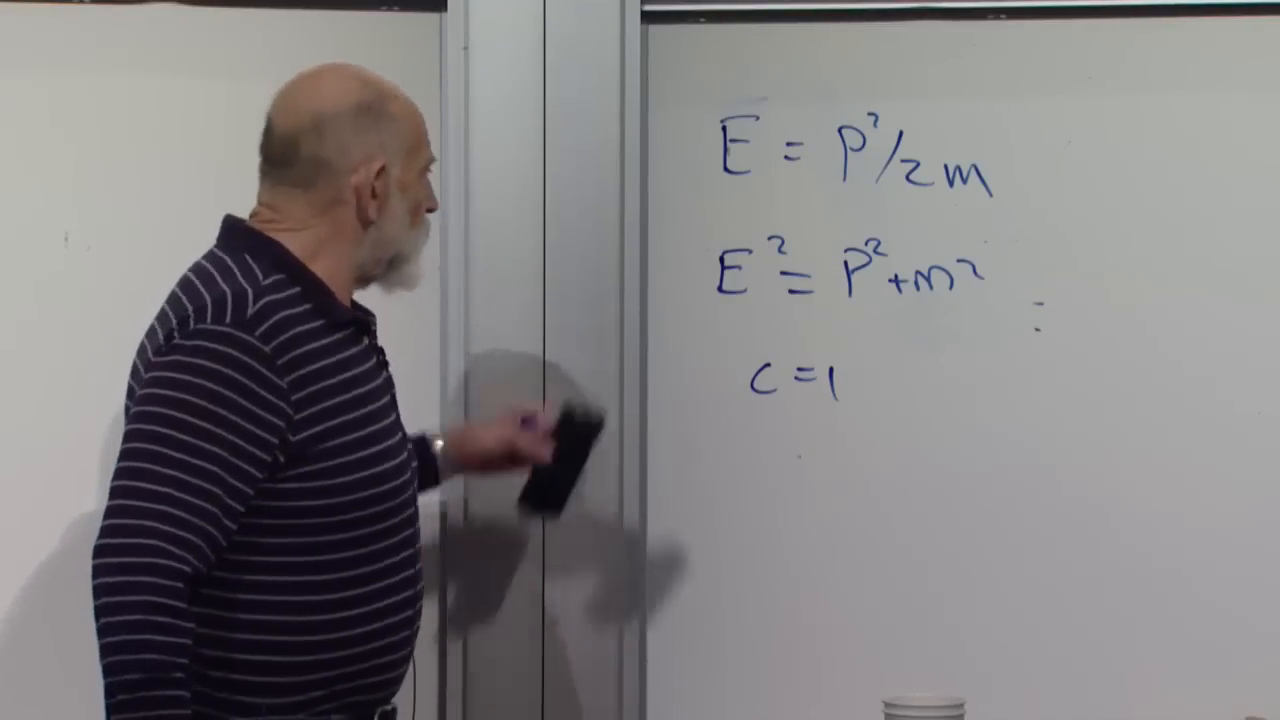
\includegraphics[width=0.94\linewidth]{lecture_09_frame_07.png}
\caption{黒板は \(E=p^2/2m\) から相対論的関係 \(E^2=p^2+m^2\) へ、\(c=1\) として移行する。}
\lectureframe{01:10:30}
\end{figure}

この置き換えを二乗した関係に適用すると
\begin{equation}
-\partial_t^2\varphi
=\left(-\partial_x^2+m^2\right)\varphi,
\label{eq:l9-klein-gordon}
\end{equation}
あるいは等価に
\begin{equation}
\left(\partial_t^2-\partial_x^2+m^2\right)\varphi=0.
\end{equation}
が得られる。これがKlein--Gordon方程式である。これは完全に意味のある相対論的場の方程式であり、特にスピンゼロの場に対してそうである。しかし、求めている電子の方程式は時間について一階でなければならない。
\begin{equation}
i\partial_t\Psi=H\Psi,
\end{equation}
すなわち、\(H^2\)だけでなく\(H\)自体が時間発展を生成するのである。

形式的に
\begin{equation}
H=\sqrt{-\partial_x^2+m^2}.
\end{equation}
を選ぶこともできよう。この平方根は運動量空間ではきれいに定義でき、そこでは\(\sqrt{p^2+m^2}\)を掛けることになるが、位置空間では非局所的な擬微分作用素である。それは技術的には意味があるものの、我々が求める局所方程式にとっては美的に役立たない。したがって、我々は再び出発する。

\section{質量ゼロの右進行波}

まず右へ進む質量ゼロの粒子を考える。その正エネルギーと運動量は
\begin{equation}
E=p
\qquad (c=1).
\end{equation}
を満たす。量子化すると
\begin{equation}
i\partial_t\psi=-i\partial_x\psi,
\end{equation}
または
\begin{equation}
(\partial_t+\partial_x)\psi=0.
\label{eq:l9-right-mover}
\end{equation}
となる。すべての解は
\begin{equation}
\psi(x,t)=f(x-t).
\end{equation}
の形をとる。その波形は剛直であり、光速で右へ進む。

直ちに二つの困難が現れる。第一に、式~\eqref{eq:l9-right-mover}を任意のフーリエモードに作用させると、負の運動量はエネルギー\(E=p<0\)をもつので、ハミルトニアンには下界がない。手で\(p>0\)に制限すれば右進行成分だけが残るが、それはまだ我々が望む電子の理論ではない。第二に、この方程式は一方通行であり、通常の左進行電子を含まない。我々はまず左右の問題を治し、負エネルギーの問題は露呈したままにしておく。

\section{二成分とアルファ行列}

二つの振幅を導入する。
\begin{equation}
\Psi(x,t)=
\begin{pmatrix}
\psi_1(x,t)\\[3pt]
\psi_2(x,t)
\end{pmatrix},
\end{equation}
ここで\(\psi_1\)は質量ゼロ極限で右進行、\(\psi_2\)は左進行である：
\begin{align}
(\partial_t+\partial_x)\psi_1&=0,
&
(\partial_t-\partial_x)\psi_2&=0.
\end{align}
量子力学ではまた、この二つの任意の重ね合わせも許される。したがって粒子は、一度きりで選ばれる古典的なラベルをもつのではなく、両方向に対する振幅をもちうる。

この余分な二値自由度は代数的にはスピンに似ているが、一次元では通常の角運動量ではない。
\begin{equation}
\alpha=
\begin{pmatrix}
1&0\\
0&-1
\end{pmatrix}
=\sigma_3.
\label{eq:l9-alpha}
\end{equation}
を定義する。その\(+1\)固有ベクトルは右進行成分を選び、\(-1\)固有ベクトルは左進行成分を選ぶ。質量ゼロの理論では、ハミルトニアンは単に
\begin{equation}
H=\alpha p,
\end{equation}
であり、二つの方程式は
\begin{equation}
i\partial_t\Psi=-i\alpha\partial_x\Psi.
\label{eq:l9-massless-dirac}
\end{equation}
にまとめられる。

\begin{classroomqa}
\lecturetimestamp{01:22:44}
\audiencequestion{二つの成分を区別する対角行列の名前は何か。}
\lecturerresponse{パウリ行列としては\(\sigma_3\)であり、\(\sigma_1\)ではない。現在の構成に対するディラックの記法では、これを\(\alpha\)と呼ぶ。その代数はよく知られたパウリ代数であるが、ここでの物理的ラベルはスピン角運動量ではなく方向である。}
\end{classroomqa}

\begin{classroomqa}
\lecturetimestamp{01:23:32}
\audiencequestion{方向がベクトルである三次元では、この構成はより幾何学的な意味をもつようになるのか。}
\lecturerresponse{はい。三次元の問題では各空間方向に対して一つの行列が必要となり、より豊かなスピノル構造へと導かれる。それでも一次元模型はそれ自身の設定において厳密であり、余分な複雑さなしに本質的な左右の代数を切り出している。}
\end{classroomqa}

\begin{figure}[htbp]
\centering
\includegraphics[width=0.94\linewidth]{lecture_09_frame_03.png}
\caption{黒板上の質量ゼロ二成分方程式：\(H=\alpha P\)。ここで対角行列は\(\psi_1\)と\(\psi_2\)に反対向きの伝播を割り当てる。}
\lectureframe{01:26:00}
\end{figure}

一方通行の問題は消えた。負エネルギーのスペクトルは残り、さらに第三の欠陥を発見した。すなわち、二つの成分は依然として質量ゼロで光速で伝播する。次の段階では静止エネルギーを導入し、方向を結合しなければならない。

\section{質量の追加とディラック代数の発見}

質量に比例する最も一般的な単純項を加える。
\begin{equation}
H=\alpha p+\beta m,
\label{eq:l9-dirac-hamiltonian}
\end{equation}
ここで\(\beta\)は二成分指数にのみ作用する。それは単位行列でも他の何らかの行列でもありえたが、相対論的分散関係に決定させる。

\(H^2\)が\(p^2+m^2\)に等しくなければならないので、式~\eqref{eq:l9-dirac-hamiltonian}を二乗する：
\begin{align}
H^2
&=(\alpha p+\beta m)^2\\
&=\alpha^2p^2+\beta^2m^2
+(\alpha\beta+\beta\alpha)pm.
\label{eq:l9-square-dirac}
\end{align}
これらの行列は\(p\)と可換である。なぜなら、それらは内部二成分空間に作用し、\(p\)は空間波動関数に作用するからである。式~\eqref{eq:l9-rel-dispersion}と一致させるには
\begin{equation}
\alpha^2=\mathbb{1},
\qquad
\beta^2=\mathbb{1},
\qquad
\{\alpha,\beta\}
=\alpha\beta+\beta\alpha=0.
\label{eq:l9-dirac-algebra}
\end{equation}
が必要である。第一の条件は\(\alpha=\sigma_3\)に対してすでに成り立つ。それとは異なるパウリ行列は、いずれもそれと反可換であり、二乗すると単位行列になる。ここでは次のように選ぶ。
\begin{equation}
\beta=
\begin{pmatrix}
0&1\\
1&0
\end{pmatrix}
=\sigma_1.
\label{eq:l9-beta}
\end{equation}
\(\sigma_2\)ではなく\(\sigma_1\)を選ぶのは基底の規約であり、どちらもユニタリな基底変換の後で同じ代数を実現する。

\begin{classroomqa}
\lecturetimestamp{01:33:00}
\audiencequestion{ディラックは、パウリ行列がこれらの代数的条件を満たすことを単に認識したのか。}
\lecturerresponse{歴史的な導出は三次元で直接行われ、必要な関係を満たす行列が導入された。条件を書き下してしまえば、パウリ代数によって一次元の解は直ちに得られる。すなわち、二つの異なるパウリ行列を選べばよい。}
\end{classroomqa}

\begin{classroomqa}
\lecturetimestamp{01:34:24}
\audiencequestion{この\(\beta\)は相対論的速度パラメータ\(v/c\)か。}
\lecturerresponse{いいえ。それはスピノル成分に作用する行列である。文字が再利用されているのはディラックの記法にすぎず、運動学的量\(v/c\)とは何の関係もない。}
\end{classroomqa}

3次元空間では、\(2\times2\)行列だけでは、必要とされる反交換行列の完全な組には不十分である。その拡張は後回しにする。1次元では、式~\eqref{eq:l9-alpha}と\eqref{eq:l9-beta}で十分である。

\section{結合した1次元ディラック方程式}

\(p=-i\partial_x\)を代入すると、ハミルトニアン形式の1次元ディラック方程式が得られる：
\begin{equation}
i\partial_t\Psi
=\left(-i\alpha\partial_x+\beta m\right)\Psi.
\label{eq:l9-one-dimensional-dirac}
\end{equation}
\(\alpha\)は対角であるから、その微分項は2つの成分を分離したまま保つ。\(\beta\)は非対角であるから、質量項はそれらを交換する。成分ごとに書くと、
\begin{align}
i\partial_t\psi_1
&=-i\partial_x\psi_1+m\psi_2,
\label{eq:l9-dirac-component-one}\\
i\partial_t\psi_2
&=+i\partial_x\psi_2+m\psi_1.
\label{eq:l9-dirac-component-two}
\end{align}

\begin{figure}[htbp]
\centering
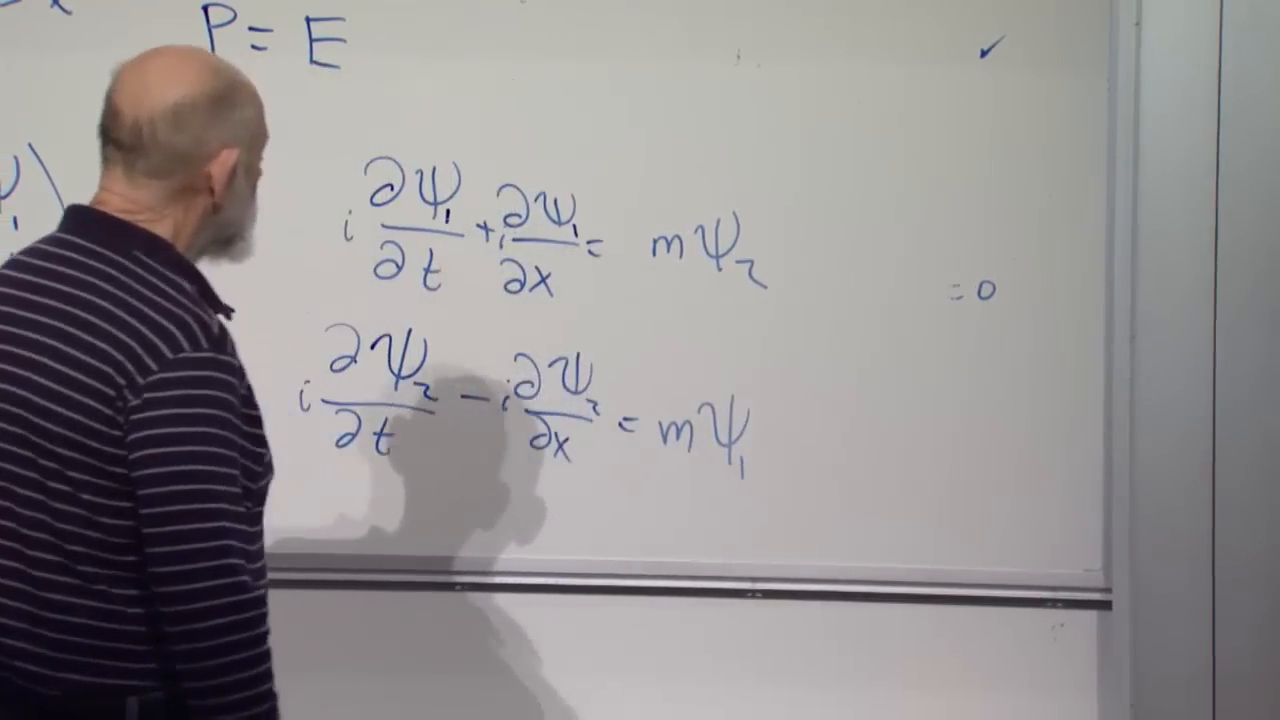
\includegraphics[width=0.94\linewidth]{lecture_09_frame_08.png}
\caption{黒板に書かれた結合成分方程式。逆符号の微分は右向きと左向きの運動を表し、非対角の質量項は\(\psi_1\)と\(\psi_2\)を入れ替える。}
\lectureframe{01:37:44}
\end{figure}

\(m\ne0\) になるとすぐに、成分は独立に発展しなくなる。一次方程式を二乗すると、各成分に対してクライン--ゴルドン演算子が回復され、
\begin{equation}
\left(\partial_t^2-\partial_x^2+m^2\right)\psi_a=0,
\qquad a=1,2,
\end{equation}
となり、平面波は \(E^2=p^2+m^2\) を満たす。その群速度は
\begin{equation}
v_g=\frac{dE}{dp}=\frac{p}{E},
\end{equation}
であり、その大きさは非零の質量に対して1未満である。

質量と左右混合の関係は偶然ではない。質量のない右向きの運動子は、任意の固有ローレンツブーストの下で右向きの運動子のままである。光速未満の観測者は光を追い越してその向きを逆にすることはできない。質量のある粒子は静止させることができ、次に同じ向きに動くより速い系から見ると、その速度は逆向きに見える。したがって、質量のある相対論的理論は右と左のセクターを永久に孤立させておくことはできない。非対角の質量項は、まさに必要な結合を与える。

\begin{classroomqa}
\lecturetimestamp{01:40:01}
\audiencequestion{2つの成分の入れ替わりはカイラル振動なのか？}
\lecturerresponse{この1次元基底では、\(\alpha\)が2つの質量のないカイラル方向を区別する。質量項は非対角であり、それらを混合するので、カイラリティはもはや保存されない。その意味で、質量項はカイラル振動の源である。}
\end{classroomqa}

\begin{classroomqa}
\lecturetimestamp{01:40:46}
\audiencequestion{なぜフェルミオンの方程式がボソンの方程式の平方根であるべきなのか？}
\lecturerresponse{そのように理解すべきではない。分散関係\(E^2=p^2+m^2\)は、統計に関係なく、すべての自由相対論的粒子に当てはまる。ディラック演算子はたまたまクライン--ゴルドン演算子の行列因子分解を与えるが、その代数的関係はフェルミオンをボソンから導くものではない。}
\end{classroomqa}

\begin{classroomqa}
\lecturetimestamp{01:41:31}
\audiencequestion{方程式は、左向きと右向きの因子への単純なスカラー因子分解に還元できるか？}
\lecturerresponse{質量のない極限でのみ、2つのカイラル方程式は独立なスカラー因子に分離する。\(m\ne0\)に対して、有用な因子分解は行列値的である：望まない交差項を取り除くのは、反交換する\(\alpha\)行列と\(\beta\)行列である。}
\end{classroomqa}

\begin{classroomqa}
\lecturetimestamp{01:42:04}
\audiencequestion{これら2つの結合方程式はすでにディラック方程式を構成しているのか？}
\lecturerresponse{はい。それらを合わせると1次元空間におけるディラック方程式であり、式~\eqref{eq:l9-one-dimensional-dirac}のコンパクトな形で等価に書ける。\(\beta\)を掛けることにより、より対称な共変的表記が得られるが、その形は後回しにする。}
\end{classroomqa}

2つの課題が意図的に未完成のまま残されている。この構成は負エネルギーを取り除いてはいない。それは両方の方向セクターに負エネルギー解を与えたので、その問題は今やより少なくではなく、より可視的になっている。そして理論は依然として1次元空間に住んでいる。負エネルギー解を解釈することと、行列代数を\(3+1\)次元に拡張することが次の段階である。
